%!TEX TS-program = xelatex
%!TEX encoding = UTF-8 Unicode
% !TEX root = ../../metm.tex

\chapter{FENOMENI OSCILLATORI}
%\begin{adjustwidth}{.19\textwidth}{0mm}

~\vfill

\begin{flushright}
		\textit{Nihil est in intellectu quod prius non fuerit in sensu}\footnote{
		Locuz. lat. \emph{niente è nell’intelletto, che prima non sia stato nei sensi},
		usata come assioma nella filosofia scolastica. Accolta da Locke nella
		sua teoria sull’origine delle idee, fu integrata da Leibniz con
		l’aggiunta \emph{nisi ipse intellectus} \emph{(eccetto l’intelletto stesso)}. --
		\url{treccani.it}}
	\end{flushright}

\bigskip

Il \emph{primo passo} che l'uomo compie, ciclicamente, verso la comprensione del
mondo sonoro che lo circonda è cambiato innumerevoli volte durante la storia degli
ultimi 3000 anni ed è sempre stato un passo mosso di pari passo con la musica,
la sua storia, la sua funzione culturale.

In Europa, solo nel novecento, possiamo segnalare differenti approcci alla
comprensione del mondo sonoro prima e dopo le guerre, prima e dopo la radio-televisione,
prima e dopo il calcolatore digitale, prima e dopo l'automobile come bene primario.

%Varese:
%Turing:

Oggi si può ascoltare e cominciare a parlare di suono cercando di unire discipline diverse
che trattano il tema scientificamente, tra cui, la musica, ormai è una di queste.
Il primo oggetto analizzabile da questo punto di vista è proprio l'oscillazione nel tempo,
il moto che da vita alla materia in vibrazione.

\clearpage

%!TEX TS-program = xelatex
%!TEX encoding = UTF-8 Unicode
%!TEX root = ../../metp.tex

\section{Oscillazioni}

Osservando, anche ad occhi chiusi, una ruota panoramica potremmo dire che
completa una rotazione ogni 30 minuti. Osservando ancora il comportamento di
questa ruota panoramica notiamo che questa compie un giro ogni 30 minuti,
ovvero completa un ciclo di rotazione tornando al punto di partenza e poi
ripete questa rivoluzione più volte. Questo è un esempio di funzione periodica,
perché la ruota panoramica ripete la sua rivoluzione, o ciclo, ogni 30 minuti
e quindi diciamo che ha un periodo di 30 minuti.

%!TEX TS-program = xelatex
%!TEX encoding = UTF-8 Unicode

%------------------------- IMMAGINE TIKZ
\begin{tikzpicture}[scale=.99]
  \draw[->] (0,-2.5) -- (0,2.5);
  \draw[->] (-2.5,0) -- (2.5,0);
       \draw[
         postaction={
         decorate,decoration={
         markings,
         mark=at position 0.19 with {\arrow[line width=1mm]{>}}}},
         thick
       ] (0,0) circle (2);
       \coordinate (A) at (2,0);
       \filldraw (A) circle (2pt) node[above right] {00'};
       \filldraw (A) circle (2pt) node[below right] {30'};
\end{tikzpicture}
%------------------------- IMMAGINE TIKZ


Osservate ancora la ruota panoramica, si muove in senso antiorario. C'è una
sola cabina occupata, seguiamola. Volendo prendere nota dell'altezza di quella
cabina durante i trenta minuti che impiega a tornare al punto di partenza,
seguendola disegneremmo una linea, probabilmente verticale, che va dall'altezza
minima all'altezza massima.

%!TEX TS-program = xelatex
%!TEX encoding = UTF-8 Unicode

%------------------------- IMMAGINE TIKZ
\begin{tikzpicture}[scale=.99]
  \draw[->] (0,-2.5) -- (0,2.5);
  \draw[->] (-2.5,0) -- (2.5,0);

\draw[
  postaction={
    decorate,decoration={
      markings,
      mark=at position 0.19 with {\arrow[line width=1mm]{>}},
      mark=at position 0.69 with {\arrow[line width=1mm]{>}}}},
    thick
] (0,0) circle (2);

\coordinate (A) at (2,0);

\filldraw (A) circle (2pt) node[above right] {00'};
\filldraw (A) circle (2pt) node[below right] {30'};

\coordinate (B) at (90 : 2);

\filldraw (B) circle (2pt) node[above left] {Cabina};

\draw (4,-2) -- (4,2);

\coordinate (C) at (4,0);
\coordinate (D) at (4,2);
\coordinate (F) at (4,-2);

\filldraw (C) circle (2pt) node[above right] {0};
\filldraw (D) circle (2pt) node[above right] {altezza massima};
\filldraw (F) circle (2pt) node[below right] {altezza minima};

\coordinate (E) at (270 : 2);

\filldraw (E) circle (2pt) node[below right] {Cabina};

\draw[dashed] (0,2) -- (4,2);
\draw[dashed] (0,-2) -- (4,-2);
\end{tikzpicture}
%------------------------- IMMAGINE TIKZ


Se decidessimo che il nostro foglio avesse non una, come nella descrizione
precedente, ma due dimensioni di rappresentazione, l'altezza ed il tempo, e
quindi seguissimo con lo sguardo la cabina ed annotando l'altezza spostassimo
simultaneamente ed a velocità costante il foglio, simulando lo scorrimento del
tempo, il disegno finale dovrebbe apparire come un'onda.

%!TEX TS-program = xelatex
%!TEX encoding = UTF-8 Unicode
%!TEX root = ../../../LSSN.tex

%------------------------- IMMAGINE TIKZ
\begin{tikzpicture}[scale=.99]
  \draw[->] (0,-2.5) -- (0,2.5);
  \draw[->] (-2.5,0) -- (2.5,0);

\draw[
  postaction={
    decorate,decoration={
      markings,
      mark=at position 0.19 with {\arrow[line width=1mm]{>}},
      mark=at position 0.69 with {\arrow[line width=1mm]{>}}}},
    thick
] (0,0) circle (2);

\coordinate (A) at (2,0);

\filldraw (A) circle (2pt) node[above left] {00'};
\filldraw (A) circle (2pt) node[below left] {30'};

\coordinate (B) at (90 : 2);

\filldraw (B) circle (2pt) node[above left] {Cabina};

\coordinate (E) at (270 : 2);

\filldraw (E) circle (2pt) node[below right] {Cabina};

\draw[dashed] (0,2) -- (6,2);
\draw[dashed] (0,-2) -- (10,-2);

  \draw[->] (3.5,-2.5) -- (3.5,2.5);
  \draw[->] (3,0) -- (10,0);

\draw[thick] (3.5,0) sin (5,2) cos (6.5,0) sin (8,-2) cos (9.5, 0);

\coordinate (F) at (5,2);
\coordinate (G) at (8,-2);

\filldraw (G) circle (2pt) node[above right] {};
\filldraw (F) circle (2pt) node[above right] {};

\end{tikzpicture}
%------------------------- IMMAGINE TIKZ


Con la rappresentazione dell'onda descriviamo un'oscillazione, ovvero un moto
periodico attorno alla posizione di equilibrio.

Un altro fenomeno oscillatorio estremamente esemplificativo è quello del pendolo.

Da un punto di quiete il pendolo si muoverà nel tempo fino al suo massimo
spostamento per poi tornare al punto di partenza e ripetere un uguale movimento
in senso opposto.

Considerando un pendolo che si sposti da una parte all'altra rispetto alla sua
posizione di equilibrio anche il suo movimento oscillatorio nel tempo può essere
rappresentato come un'oscillazione.

%!TEX TS-program = xelatex
%!TEX encoding = UTF-8 Unicode
%!TEX root = ../../../LSSN.tex

%------------------------- IMMAGINE TIKZ
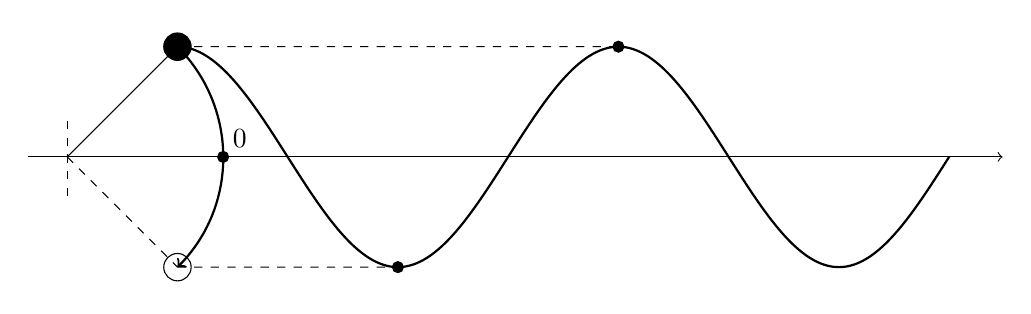
\begin{tikzpicture}[scale=.99]
  \draw[dashed] (0,-0.5) -- (0,0.5);
  \draw[->] (-0.5,0) -- (12,0);
       %\draw[thick] (0,0) circle (2);
       \draw[thick, ->] (45:2)arc(45:-45:2);
       \coordinate (origin) at (0:0);
       \coordinate (A) at (45:2);
       \coordinate (B) at (-45:2);
       \coordinate (0) at (0:2);
       \coordinate (1) at (7.071,1.414);
       \coordinate (-1) at (4.242,-1.414);
  \filldraw (A) circle (2pt) node[above right] {};
  \filldraw (0) circle (2pt) node[above right] {0};
  \filldraw (A) circle (5pt) node[above right] {};
  \draw (B) circle (5pt) node[above right] {};
  \draw[-] (origin) -- (A);
  \draw[dashed] (origin) -- (B);
  \draw[dashed] (B) -- (-1);
  \draw[dashed] (A) -- (1);
  \filldraw (1) circle (2pt) node[above] {};
  \filldraw (-1) circle (2pt) node[below] {};

  \draw[thick] (A) cos (2.828,0) sin (4.242,-1.414) cos (5.656, 0) sin (7.071,1.414) cos (8.485,0) sin (9.899,-1.414) cos (11.313,0);
\end{tikzpicture}
%------------------------- IMMAGINE TIKZ


L'oscillazione rappresentata da un moto di questo tipo è definita moto armonico
semplice o sinusoidale.

Definiamo una quantità in oscillazione quando il suo valore si muove con
continuità passando tra un massimo ad un minimo.

\clearpage

\section{Le grandezze di un'oscillazione}

La rappresentazione di un fenomeno oscillatorio ci permette di descrivere
quali siano le grandezze principali:

\begin{compactitem}
	\item ampiezza
	\item frequenza
	\item periodo
	\item fase (da spiegare)
	\item lunghezza d'onda (da spiegare)
	%\item pulsazione
\end{compactitem}

Definiamo \textbf{ampiezza} di un'oscillazione il massimo valore raggiunto
dal suo valore di equilibrio.

Facendo riferimento al movimento del pendolo, diciamo che la distanza massima
raggiunta nel suo movimento da una parte all'altra rispetto alla posizione di
equilibrio definisce la sua ampiezza di oscillazione.

%!TEX TS-program = xelatex
%!TEX encoding = UTF-8 Unicode
%!TEX root = ../../../LSSN.tex

%------------------------- IMMAGINE TIKZ
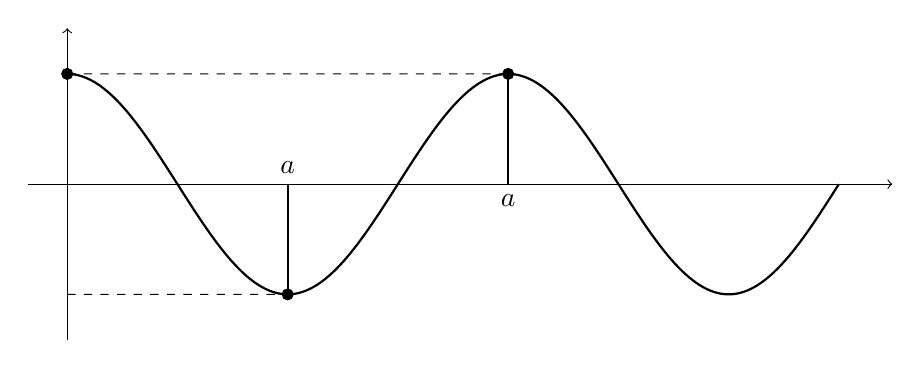
\begin{tikzpicture}[scale=.99]
  \draw[->] (1.414,-2) -- (1.414,2);
  \draw[->] (0.914,0) -- (12,0);
       \coordinate (origin) at (0:0);
       \coordinate (A) at (45:2);
       \coordinate (B) at (-45:2);
       \coordinate (0) at (0:2);
       \coordinate (1) at (7.071,1.414);
       \coordinate (-1) at (4.242,-1.414);
  \filldraw (A) circle (2pt) node[above right] {};
  \draw[dashed] (B) -- (-1);
  \draw[dashed] (A) -- (1);
  \filldraw (1) circle (2pt) node[above] {};
  \filldraw (-1) circle (2pt) node[below] {};

  \draw[thick] (1.414,1.414) cos (2.828,0) sin (4.242,-1.414) cos (5.656, 0) sin (7.071,1.414) cos (8.485,0) sin (9.899,-1.414) cos (11.313,0);

  \draw[thick] (4.242,-1.414) -- (4.242,0) node[above] {$a$};
  \draw[thick] (7.071,1.414) -- (7.071,0) node[below] {$a$};
\end{tikzpicture}
%------------------------- IMMAGINE TIKZ


Definiamo \textbf{frequenza} il numero di ripetizioni nell'unità di tempo. La
frequenza di oscillazione di un pendolo corrisponde al numero di volte che questo
torna alla posizione di partenza dopo aver percorso l'intero tragitto ondulatorio.
Nell'immagine della ruota panoramica la frequenza descrive quanti giri essa realizza
nell'unità di tempo prestabilita.

Descriviamo quindi con il valore di \textbf{frequenza} di un'oscillazione il
\emph{numero di cicli per secondo (cps)}. L'unità di misura della frequenza è
\emph{Hertz (Hz)}.

%!TEX TS-program = xelatex
%!TEX encoding = UTF-8 Unicode

%------------------------- IMMAGINE TIKZ
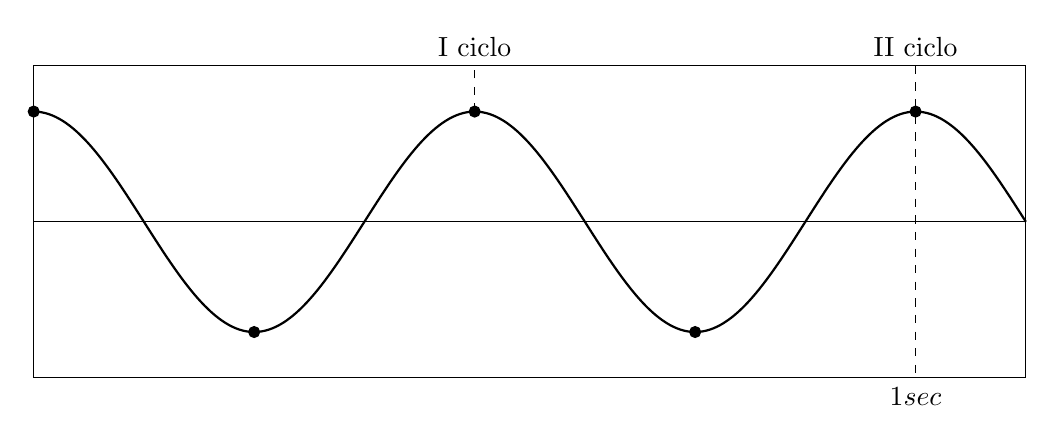
\begin{tikzpicture}[scale=.99]
  \draw[] (1.414,-2) rectangle (14.142,2);
  \draw[dashed] (12.727,2) -- (12.727,-2) node[below]{1$sec$};
  \draw[-] (1.414,0) -- (14.142,0);
       \coordinate (origin) at (0:0);
       \coordinate (A) at (45:2);
       \coordinate (-1) at (4.242,-1.414);
       \coordinate (1) at (7.071,1.414);
       \coordinate (-1b) at (9.899,-1.414);
       \coordinate (1b) at (12.727,1.414);
  \filldraw (A) circle (2pt) node[above right] {};
  \filldraw (1) circle (2pt) node[above] {};
  \filldraw (-1) circle (2pt) node[below] {};
  \filldraw (1b) circle (2pt) node[below] {};
  \filldraw (-1b) circle (2pt) node[below] {};

  \draw[dashed] (7.071,1.414) -- (7.071,2) node[above]{I ciclo};
  \draw[] (12.727,2) -- (12.727,2) node[above]{II ciclo};

  \draw[thick] (1.414,1.414) cos (2.828,0) sin (4.242,-1.414) cos (5.656, 0) sin (7.071,1.414) cos (8.485,0) sin (9.899,-1.414) cos (11.313,0) sin (12.727,1.414) cos (14.142,0);
\end{tikzpicture}
%------------------------- IMMAGINE TIKZ


Il \emph{ciclo} o \textbf{periodo} di un'oscillazione rappresenta la durata di
una singola oscillazione alla frequenza data.
Il legame tra frequenza e periodo è tale che all'aumentare della frequenza
diminuisce la durata, e quindi il periodo, nel rapporto di $T = 1/f$ dove
$T$ è la durata del periodo espressa in secondi.

Considerando quindi il \emph{secondo} un intero divisibile in parti uguali,
definiamo con $f$ la \emph{frequenza}, ovvero il numero di parti e con $T$
il \emph{periodo} ovvero la durata di una singola parte. La durata della
singola parte moltiplicata per il numero delle parti ri-compone l'intero \emph{secondo}.

\bigskip

%------------------------- APPROFONDIMENTO
		\begin{tabular}{L{.969\textwidth}}%
		\toprule
			\textbf{Hertz}\\
		\midrule
			Unità di misura della frequenza dei fenomeni periodici; un fenomeno ha
			frequenza 1 \emph{Hertz} se un suo periodo dura 1 secondo; simbolo
			\emph{Hz}.\\

			DATA 1937.\\

			ETIMOLOGIA Dal nome del fisico tedesco Heinrich Rudolf Hertz (1857–94),
			Fisico tedesco e pioniere della comunicazione radio. Ha proseguito il
			lavoro di Maxwell sulle onde elettromagnetiche e fu il primo a trasmettere
			e ricevere onde radio. Hertz ha anche dimostrato che la luce ed il calore
			radiante hanno natura elettromagnetica. \\
		\bottomrule
		\end{tabular}
%------------------------- APPROFONDIMENTO

\clearpage

\section{Oscillazione Sinusoidale}

%------------------------- APPROFONDIMENTO
		\begin{tabular}{L{.969\textwidth}}%
		\toprule
			\textbf{Sinusoide} \\
		\midrule
			In geometria: curva sinusoide (o la sinusoide s.f.), la curva che, in
			coordinate cartesiane ortogonali, rappresenta il diagramma della funzione
			seno, tipico dei fenomeni periodici senza smorzamento. \\

			DATA 1895.\\

			ETIMOLOGIA Der. del lat. \emph{sinus -us} ‘seno’, col suff. \emph{-oide}.\\
		\bottomrule
		\end{tabular}
%------------------------- APPROFONDIMENTO

% %!TEX TS-program = xelatex
%!TEX encoding = UTF-8 Unicode
%!TEX root = ../../../LSSN.tex

%------------------------- IMMAGINE TIKZ
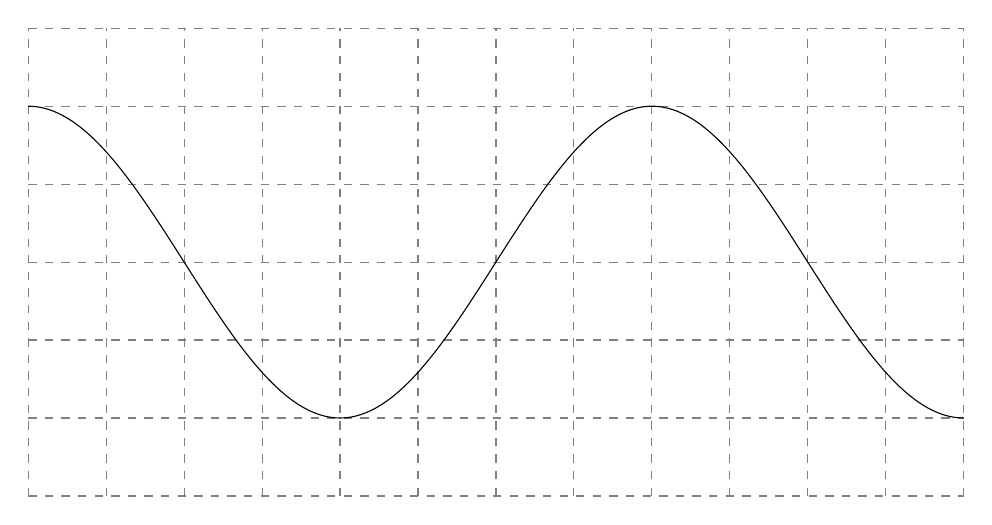
\begin{tikzpicture}[scale=.99]
   \draw[dashed, gray] (0,-3) grid (12,3);
   %\draw[help lines] (0,-3) grid (12,3);
   \draw (0,2) cos (2,0) sin (4,-2) cos (6,0) sin (8,2) cos (10,0) sin (12,-2);
   %%\draw (0,0) to (12,0);
\end{tikzpicture}
%------------------------- IMMAGINE TIKZ

%
% Potremmo rapidamente intuire la connessione  con il cerchio unitario, poiché
% l'altezza della cabina corrisponderebbe al valore $ y $ di un punto sul cerchio.
% Possiamo determinare il valore di $ y $ usando la funzione seno. Per avere
% un'idea migliore del comportamento di questa funzione, possiamo creare una
% tabella di valori che conosciamo e usarli per tracciare un grafico delle
% funzioni seno e coseno.
%
% %!TEX TS-program = xelatex
%!TEX encoding = UTF-8 Unicode
%!TEX root = ../../../LSSN.tex

%------------------------- IMMAGINE TIKZ
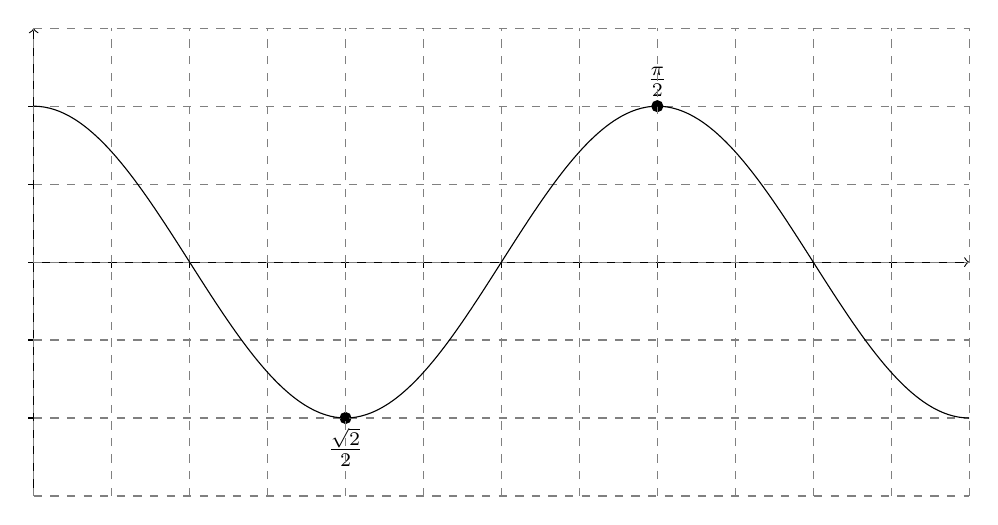
\begin{tikzpicture}[scale=.99]

    \draw[->] (0,-3) -- (0,3);
    \draw[->] (0,0) -- (12,0);
    \foreach \x in {1,2,3,4,5,6,7,8,9,10,11}
        \draw (\x,2pt) -- (\x,-2pt);
    \foreach \y in {-2,-1,0,1,2}
        \draw (2pt,\y) -- (-2pt,\y);

\coordinate (A) at (8,2);
\coordinate (B) at (4,-2);
\filldraw (A) circle (2pt) node[above] {{$\frac{\pi}{2}$}};
\filldraw (B) circle (2pt) node[below] {{{$\frac{\sqrt2}{2}$}}};

   \draw[dashed, gray] (0,-3) grid (12,3);
   %\draw[help lines] (0,-3) grid (12,3);
   \draw (0,2) cos (2,0) sin (4,-2) cos (6,0) sin (8,2) cos (10,0) sin (12,-2);
   %%\draw (0,0) to (12,0);
   \label{sin001}
\end{tikzpicture}
%------------------------- IMMAGINE TIKZ

%
% %!TEX TS-program = xelatex
%!TEX encoding = UTF-8 Unicode
%!TEX root = ../../../LSSN.tex

%------------------------- IMMAGINE TIKZ
\begin{tikzpicture}[scale=1.98]
\Base
\draw [white] (-0.5,-0.5) rectangle (5.5,5.5);
\filldraw[
	thick,
	%draw=blue,
	fill=gray!40,
	fill opacity=0.3,
	text opacity=1
	]
  (O) -- (aux1) -- node[left] {$\sin x$} (aux2)  -- node[below] {$\cos x$} cycle;
\end{tikzpicture}
%------------------------- IMMAGINE TIKZ

%
% 		\begin{tabularx}{.81\textwidth}{XXXXXXXXXX}%
% 		\toprule
% 			$\theta$ & $0$ & {$\frac{\pi}{6}$} & {$\frac{\pi}{4}$} & {$\frac{\pi}{6}$} & {$\frac{\pi}{2}$} &
% 				{$\frac{2\pi}{3}$} & {$\frac{3\pi}{4}$} & {$\frac{5\pi}{6}$} & $\pi$ \\
% 		\midrule
% 			$\cos$ & $1$ & {$\frac{\sqrt{3}}{2}$} & {$\frac{\sqrt{2}}{2}$} & {$\frac{1}{2}$} & $0$ &
% 				{$-\frac{1}{2}$} & {$-\frac{\sqrt{2}}{2}$} & {$-\frac{\sqrt{3}}{2}$} & $-1$\\
% 		\midrule
% 			$\sin$ & $0$ & {$\frac{1}{2}$} & {$\frac{\sqrt{2}}{2}$} & {$\frac{\sqrt{3}}{2}$} & $1$ & {$\frac{\sqrt{3}}{2}$} &
% 				{$\frac{\sqrt{2}}{2}$} & {$\frac{1}{2}$} & $0$ \\
% 		\bottomrule
% 		\end{tabularx}
%
% %------------------------- APPROFONDIMENTO
% 		\begin{tabular}{L{1\textwidth}}%
% 		\toprule
% 			\textbf{Funzione Periodica} \\
% 		\midrule
% 			Una funzione periodica è una funzione che ripete il proprio comportamento
% 			su tutto il proprio campo d'appartenenza.
%
% 			È la funzione per cui uno spostamento orizzontale $ P $ risulta nella
% 			funzione $ f (x + P) = f (x) $ per tutti i valori di $ x $.
%
% 			Quando ciò si verifica indichiamo il più piccolo spostamento orizzontale
% 			di questo tipo, con $ P > 0 $, il
% 			periodo della funzione. \\
% 		\bottomrule
% 		\end{tabular}
% %------------------------- APPROFONDIMENTO
%
% \lstinputlisting
% [%style      = SuperCollider-IDE,
%   basicstyle = \ttfamily\footnotesize,
%   caption    = {CSOUND - Onda sinusoidale 440Hz}
% ]{CAPITOLI/CODES/2000/sinusoide.csd}
%
% %------------------------- APPROFONDIMENTO
% 		\begin{tabular}{L{1\textwidth}}%
% 		\toprule
% 			\textbf{Oscillatore}\\
% 		\midrule
% 		Apparecchio atto a provocare variazioni periodiche (oscillazioni) di una o
% 		più grandezze fisiche
%
% 		Oscillatore elettrico, che provoca variazioni periodiche di grandezze
% 		elettriche (correnti o tensioni); secondo la forma delle oscillazioni
% 		(segnali) prodotte può essere sinusoidale, a onda rettangolare, ecc.,
% 		secondo la frequenza a bassa, a media, ad alta frequenza, oppure a microonde,
% 		secondo il principio di funzionamento a triodo, a reazione, a cavità risonante,
% 		piezoelettrico, ecc.
%
% 		Oscillatore meccanico, che induce deformazioni o spostamenti periodici di
% 		grandezze meccaniche (part. : o. armonico, se le oscillazioni sono
% 		sinusoidali, come quelle provocate da una forza di richiamo proporzionale
% 		allo spostamento e di segno opposto).\\
%
% 		DATA 1897 \\
% 		\bottomrule
% 		\end{tabular}
% %------------------------- APPROFONDIMENTO

\clearpage

